\documentclass{article}
\usepackage{amsmath}
\usepackage{amssymb}
\usepackage{graphicx}
\usepackage{hyperref}
\usepackage[version=4]{mhchem}

\title{Example 15}
\date{}

\begin{document}
\maketitle

Prove the Menelaus' Theorem: A line intersects the sides or extension of the sides \(A B, B C\) and \(C A\) of \(\triangle A B C\) at \(X, Y\) and \(Z\), respectively. The following holds \(\frac{A X}{B X} \cdot \frac{B Y}{C Y} \cdot \frac{C Z}{A Z}=1\)

Proof:
\begin{center}
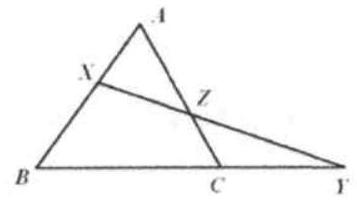
\includegraphics[width=\textwidth]{images/problem_image_1.jpg}
\end{center}

Draw \(C G / / X Y\) to meet \(A B\) at \(G\).\\
Since \(\triangle B Y X \sim \triangle B C G\), we have \(\frac{B Y}{C Y}=\frac{B X}{G X}\)\\
\centering
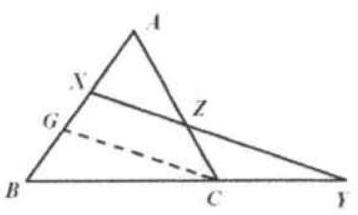
\includegraphics[width=\textwidth]{images/reasoning_image_1.jpg}

Since \(\triangle A G C \sim \triangle A X Z\), we have \(\frac{C Z}{A Z}=\frac{G X}{A X}\) (2)\\
(1) \(\times\) (2): \(\frac{B Y}{C Y} \times \frac{C Z}{A Z}=\frac{B X}{G X} \times \frac{G X}{A X}=\frac{B X}{A X}\), or \(\frac{A X}{B X} \cdot \frac{B Y}{C Y} \cdot \frac{C Z}{A Z}=1\).



\end{document}
